% Options for packages loaded elsewhere
\PassOptionsToPackage{unicode}{hyperref}
\PassOptionsToPackage{hyphens}{url}
%
\documentclass[
]{article}
\usepackage{lmodern}
\usepackage{amssymb,amsmath}
\usepackage{ifxetex,ifluatex}
\ifnum 0\ifxetex 1\fi\ifluatex 1\fi=0 % if pdftex
  \usepackage[T1]{fontenc}
  \usepackage[utf8]{inputenc}
  \usepackage{textcomp} % provide euro and other symbols
\else % if luatex or xetex
  \usepackage{unicode-math}
  \defaultfontfeatures{Scale=MatchLowercase}
  \defaultfontfeatures[\rmfamily]{Ligatures=TeX,Scale=1}
\fi
% Use upquote if available, for straight quotes in verbatim environments
\IfFileExists{upquote.sty}{\usepackage{upquote}}{}
\IfFileExists{microtype.sty}{% use microtype if available
  \usepackage[]{microtype}
  \UseMicrotypeSet[protrusion]{basicmath} % disable protrusion for tt fonts
}{}
\makeatletter
\@ifundefined{KOMAClassName}{% if non-KOMA class
  \IfFileExists{parskip.sty}{%
    \usepackage{parskip}
  }{% else
    \setlength{\parindent}{0pt}
    \setlength{\parskip}{6pt plus 2pt minus 1pt}}
}{% if KOMA class
  \KOMAoptions{parskip=half}}
\makeatother
\usepackage{xcolor}
\IfFileExists{xurl.sty}{\usepackage{xurl}}{} % add URL line breaks if available
\IfFileExists{bookmark.sty}{\usepackage{bookmark}}{\usepackage{hyperref}}
\hypersetup{
  pdftitle={Methods/Results},
  hidelinks,
  pdfcreator={LaTeX via pandoc}}
\urlstyle{same} % disable monospaced font for URLs
\usepackage[margin=1in]{geometry}
\usepackage{longtable,booktabs}
% Correct order of tables after \paragraph or \subparagraph
\usepackage{etoolbox}
\makeatletter
\patchcmd\longtable{\par}{\if@noskipsec\mbox{}\fi\par}{}{}
\makeatother
% Allow footnotes in longtable head/foot
\IfFileExists{footnotehyper.sty}{\usepackage{footnotehyper}}{\usepackage{footnote}}
\makesavenoteenv{longtable}
\usepackage{graphicx}
\makeatletter
\def\maxwidth{\ifdim\Gin@nat@width>\linewidth\linewidth\else\Gin@nat@width\fi}
\def\maxheight{\ifdim\Gin@nat@height>\textheight\textheight\else\Gin@nat@height\fi}
\makeatother
% Scale images if necessary, so that they will not overflow the page
% margins by default, and it is still possible to overwrite the defaults
% using explicit options in \includegraphics[width, height, ...]{}
\setkeys{Gin}{width=\maxwidth,height=\maxheight,keepaspectratio}
% Set default figure placement to htbp
\makeatletter
\def\fps@figure{htbp}
\makeatother
\setlength{\emergencystretch}{3em} % prevent overfull lines
\providecommand{\tightlist}{%
  \setlength{\itemsep}{0pt}\setlength{\parskip}{0pt}}
\setcounter{secnumdepth}{-\maxdimen} % remove section numbering
\newlength{\cslhangindent}
\setlength{\cslhangindent}{1.5em}
\newenvironment{cslreferences}%
  {\setlength{\parindent}{0pt}%
  \everypar{\setlength{\hangindent}{\cslhangindent}}\ignorespaces}%
  {\par}

\title{Methods/Results}
\author{}
\date{\vspace{-2.5em}}

\begin{document}
\maketitle

\hypertarget{methods}{%
\section{Methods}\label{methods}}

\hypertarget{population}{%
\subsection{Population}\label{population}}

We present a spatial explicit stochastic agent based model that
recreates the day to day dynamics in a typical nursery home during the
COVID pandemic in the United States. We use an hourly time step
resolution and we ran the model for 150 days.

\hypertarget{population-structure}{%
\subsubsection{Population structure}\label{population-structure}}

We used the floor plans and satellite imagery to recreate the spatial
structure of a typical nursery home in the US (figure 1). The nursery
home consist on 58 bedrooms designated for the residents, recreation
areas (such as dining room, and activities rooms), and rooms for staff
use. In the initial conditions there are 3 residents per room (total
174) and 170 staff divided into 3 different turns. The decision on the
population distribution was based on information obtained from an
interview with a nursery home in California.

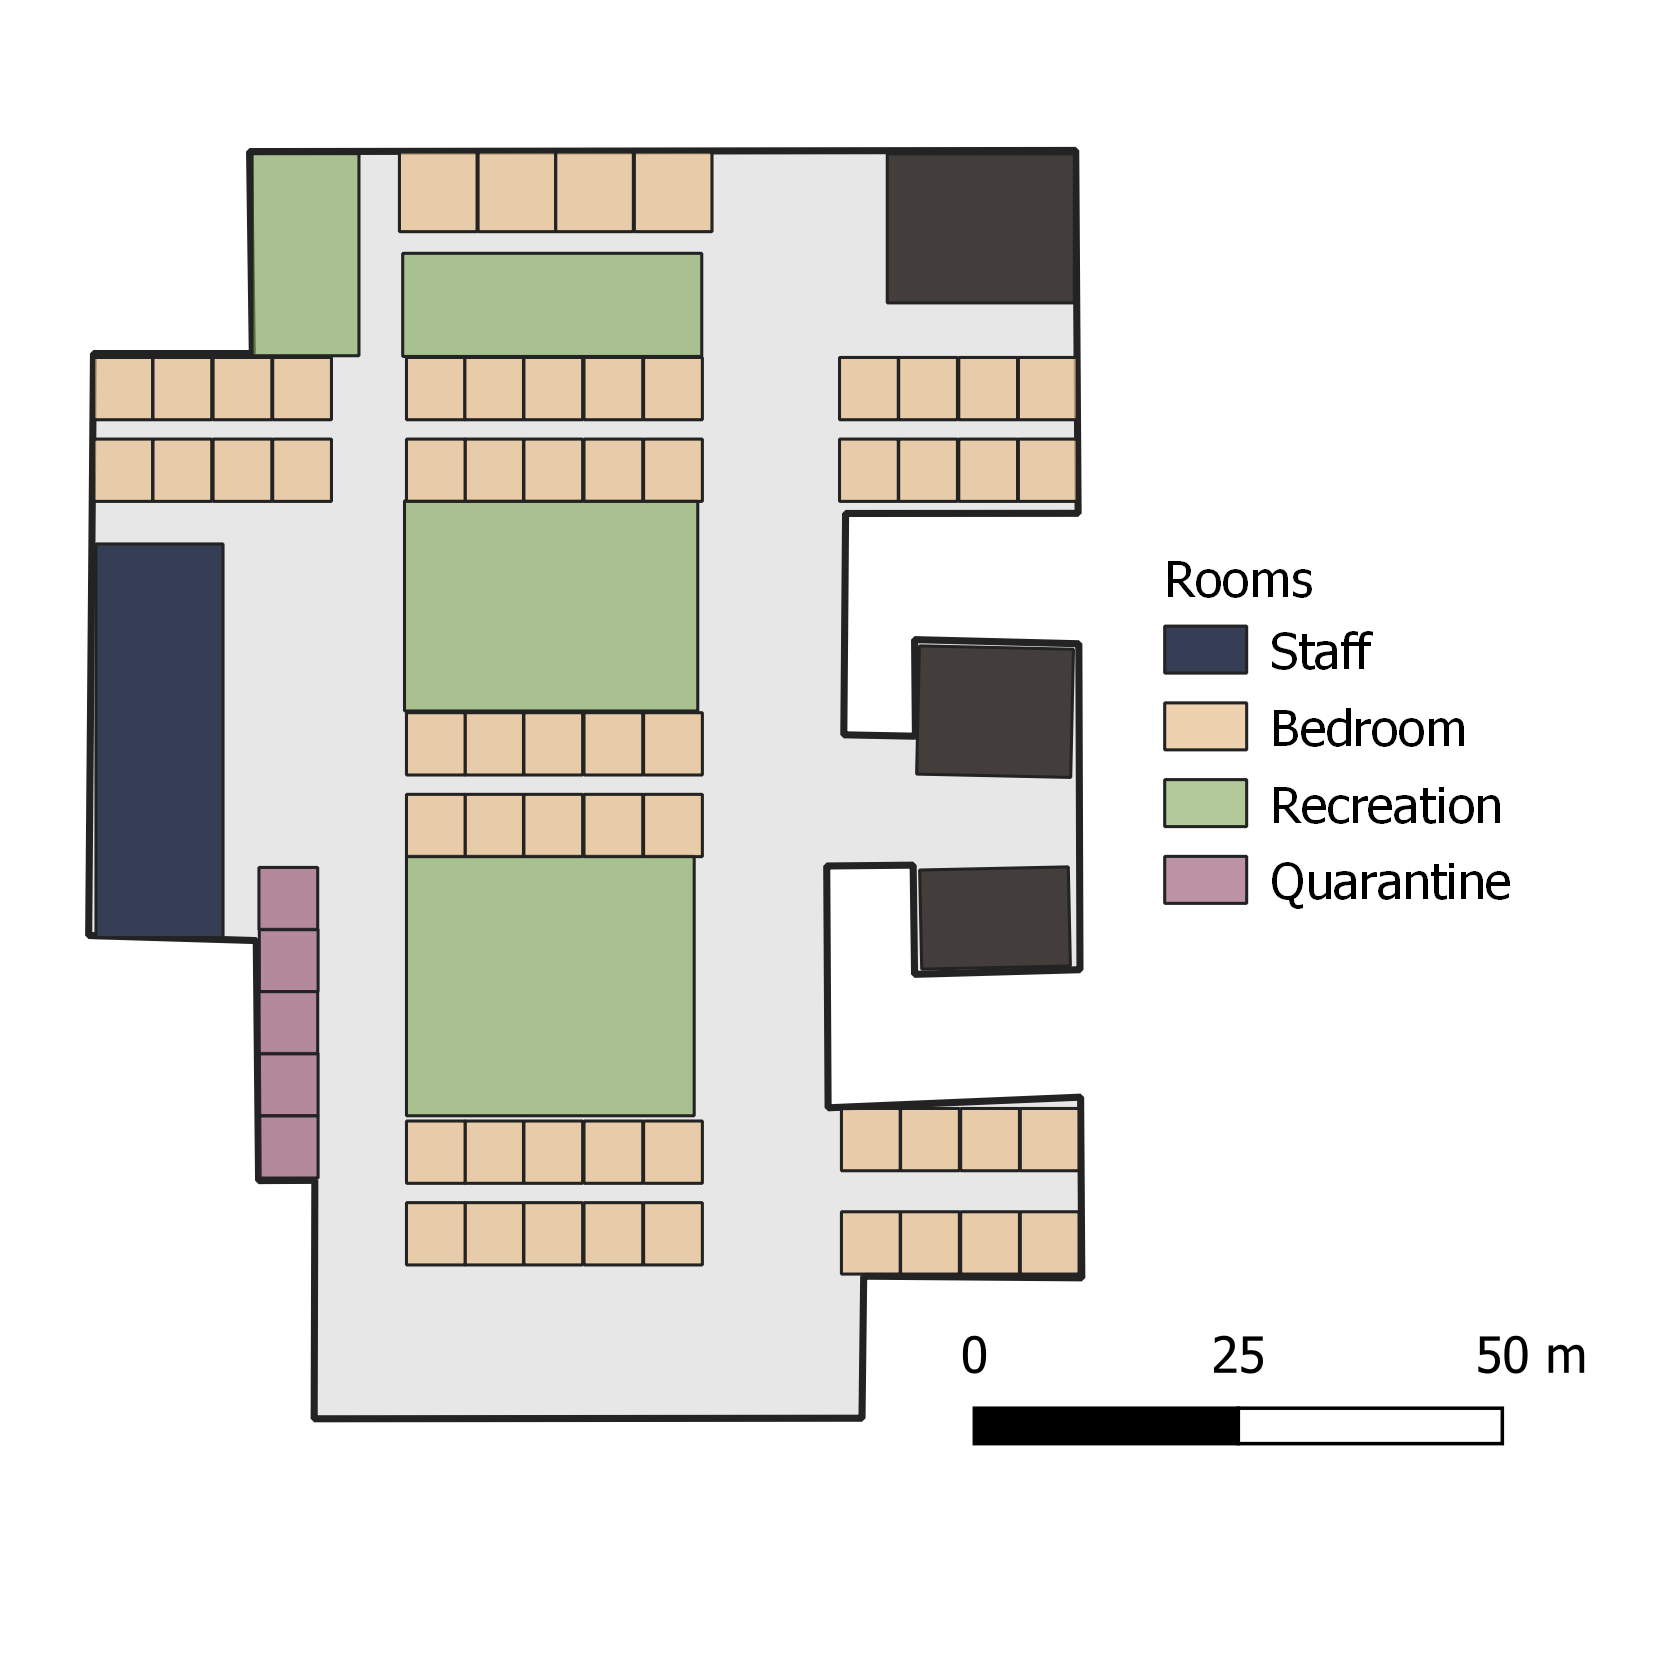
\includegraphics{Figures/NH_B}

\hypertarget{population-dynamics}{%
\subsubsection{Population dynamics}\label{population-dynamics}}

In our simulation, an agent can interact with other agents based on its
location. Given the current guidelines of recommendations for long term
care facilities, there are no visitations and the residents spend most
of the day in their rooms, so they can only interact with their
roommates and the staff. In our model each resident will have at least
one interaction with the staff per day which is based on different
contact rates depending on the staff type (CN, RN, LPN), The staff will
have different contact rates that were parametrized according on the
average number of resident contacts in a normal day (REFERENCE: Table
shared via email??). The contact rates are presented in table from
supplementary materials.

The staff agents are assigned to one of 3 different work schedules
(morning, afternoon or night) and they spend 8 hours inside the nursery
home and the rest of the time outside in the community. We only follow
the agents inside the nursery home and when the agents are outside we
assume that they all have the same probability of contacting other
people.

\hypertarget{disease-dynamics}{%
\subsubsection{Disease dynamics:}\label{disease-dynamics}}

The transmission between agents inside the facility will depend on two
parts, which are the probability that a person will shed the virus and
the probability that another person will get the virus. We decided on
model the transmission this way to represent scenarios where the
infected and susceptible could have different combination of
interventions (i.e.~only infected received the intervention, only
susceptible received the intervention, both received the intervention,
etc..). The parametrization of the transmission parameters was based on
observed outbreaks in nursery homes in California.

The introduction from the community to the facility depends on a
parameter \emph{Introduction\_p} that represents how likely is that a
staff agent will be infected in the community.

All the agents start as susceptible and after 1 day there is a resident
introduced with the disease. Then we follow up for 150 days or until the
disease has been absent for more than 14 simulation days. Once the
transmission between a infectious agent to a susceptible agent has been
successful, the susceptible agent becomes exposed and based on a
distribution for the latent period \(\lambda\), the agent becomes
infectious after \(\lambda\) number of days, which can be either
symptomatic and asymptomatic. The agent can infect other agents only
when its in the Infectious state, then they remain infectious during 15
days and they transition to recovered. The agents can transition to
infectious to hospitalized at any moment based on the hospitalization
rate. When the agents has been recovered they acquire infection
immunity, which lasts for 120 days.

\includegraphics{Figures/DiseaseDynamics}

Transmission parameters:

\begin{longtable}[]{@{}lll@{}}
\toprule
Name & Value & Reference\tabularnewline
\midrule
\endhead
Latent period (\(\lambda\)) & \(Lognormal(7, 3)\) & (He et al.
2020)\(^{b,c}\)\tabularnewline
Shedding probability & \(0.4\) & \(^a\)\tabularnewline
Infection probability & \(0.4\) & \(^a\)\tabularnewline
Introduction probability & \(0.01\) & \(^a\)\tabularnewline
Asymptomatic probability & \(0.25\) & \(^a\)\tabularnewline
Infection duration & \(15\ days\) &\tabularnewline
Hospitalization rate & \(0.11\) &\tabularnewline
\bottomrule
\end{longtable}

\(^a\)Explored for sensitivity analysis and scenario modeling,
\(^b\)truncated distribution between a boundary of reasonable values,
\(^c\)fitted to a distribution

\hypertarget{interventions}{%
\subsection{Interventions}\label{interventions}}

We explore 3 different COVID-19 control strategies and the combination
of them. Each of the interventions have an impact in the transmission of
the disease, interventions such as the use of PPE and vaccination
reduces the probability of transmission affecting directly the
\emph{Shedding} and \emph{Infection probability}, while the isolation
affects the transmission indirectly stopping the agent to interact with
other agents. The equation 1 shows the effect of \emph{PPE effect} and
\emph{Vaccine effect} on the transmission probability, where
\(odds_\omega\) represent the global transmission probability for all
agents, \(OR_\gamma\) represent the odds ratio for the \emph{PPE
effect}, and \(OR\pi\) is the \emph{Vaccine effect}. This probability is
computed for all agents at each step so we can have different
probabilities of transmission based on the interventions each individual
received.

\[p_T = \frac{e^{\ln(odds_\omega) + \ln(OR_\pi)+ \ln(OR_\upsilon)}}{1 + e^{\ln(odds_\omega) + \ln(OR_\pi)+ \ln(OR_\upsilon)}}\]
For the implementation of the vaccination, we specified by the
proportion of residents and staff vaccinated, and a fixed interval
between the first and second dose. Then the vaccination immunity will
have a decay of 120 days and the individual will no longer have the
vaccination immunity protective effect.

Since there is still some uncertainty in the effect of the use of PPE
and the vaccine for older population, we started with values that are
within the range of reported values and then varied these values for the
sensitivity analysis and scenario modeling.

\hypertarget{testing-and-isolation}{%
\subsubsection{Testing and isolation}\label{testing-and-isolation}}

Our model represents the testing of the population with 2 different
approaches:

\begin{itemize}
\tightlist
\item
  Passive, individuals are tested once that they present symptoms, this
  approach is focused on the early detection of symptomatic individuals.
\item
  Active, a proportion of individuals are tested with a given frequency.
  In baseline scenario, 1 resident per room and all the staff are tested
  weekly. If 1 of the residents in a room is detected positive, the rest
  of the residents in that room are also tested.
\end{itemize}

Once a individual has been detected positive is isolated. There are
special isolation rooms for the residents and in the case of the staff
they are sent home. Once the individual is tested negative it return to
the facility.

Interventions parameters:

\begin{longtable}[]{@{}lll@{}}
\toprule
\begin{minipage}[b]{0.42\columnwidth}\raggedright
Name\strut
\end{minipage} & \begin{minipage}[b]{0.33\columnwidth}\raggedright
Value\strut
\end{minipage} & \begin{minipage}[b]{0.16\columnwidth}\raggedright
Reference\strut
\end{minipage}\tabularnewline
\midrule
\endhead
\begin{minipage}[t]{0.42\columnwidth}\raggedright
Test detection probability\strut
\end{minipage} & \begin{minipage}[t]{0.33\columnwidth}\raggedright
\(75\%\)\strut
\end{minipage} & \begin{minipage}[t]{0.16\columnwidth}\raggedright
\(^a\)\strut
\end{minipage}\tabularnewline
\begin{minipage}[t]{0.42\columnwidth}\raggedright
Proportion of Staff tested\strut
\end{minipage} & \begin{minipage}[t]{0.33\columnwidth}\raggedright
\(90\%\)\strut
\end{minipage} & \begin{minipage}[t]{0.16\columnwidth}\raggedright
\(^a\)\strut
\end{minipage}\tabularnewline
\begin{minipage}[t]{0.42\columnwidth}\raggedright
Proportion of Residents tested\strut
\end{minipage} & \begin{minipage}[t]{0.33\columnwidth}\raggedright
\(33.3%
\)\strut
\end{minipage} & \begin{minipage}[t]{0.16\columnwidth}\raggedright
\(^a\)\strut
\end{minipage}\tabularnewline
\begin{minipage}[t]{0.42\columnwidth}\raggedright
Frequency of testing\strut
\end{minipage} & \begin{minipage}[t]{0.33\columnwidth}\raggedright
Weekly\strut
\end{minipage} & \begin{minipage}[t]{0.16\columnwidth}\raggedright
\(^a\)\strut
\end{minipage}\tabularnewline
\begin{minipage}[t]{0.42\columnwidth}\raggedright
PPE Effect (\(OR_\pi\))\strut
\end{minipage} & \begin{minipage}[t]{0.33\columnwidth}\raggedright
0.34089\strut
\end{minipage} & \begin{minipage}[t]{0.16\columnwidth}\raggedright
(Chu et al. 2020)\(^a\)\strut
\end{minipage}\tabularnewline
\begin{minipage}[t]{0.42\columnwidth}\raggedright
Vaccine effect first and second dose (\(OR_\upsilon\))\strut
\end{minipage} & \begin{minipage}[t]{0.33\columnwidth}\raggedright
\(60\%\),\(90\%\)\strut
\end{minipage} & \begin{minipage}[t]{0.16\columnwidth}\raggedright
(Pfizer-BioNTech 2020)\(^a\)\strut
\end{minipage}\tabularnewline
\begin{minipage}[t]{0.42\columnwidth}\raggedright
Vaccine immunity duration\strut
\end{minipage} & \begin{minipage}[t]{0.33\columnwidth}\raggedright
\(120\ days\)\strut
\end{minipage} & \begin{minipage}[t]{0.16\columnwidth}\raggedright
\(^a\)\strut
\end{minipage}\tabularnewline
\bottomrule
\end{longtable}

\(^a\)Explored for sensitivity analysis and scenario modeling,
\(^b\)truncated distribution between a boundary of reasonable values,
\(^c\)fitted to a distribution

\hypertarget{scenario-modeling}{%
\subsubsection{Scenario modeling}\label{scenario-modeling}}

To asses the effect of different combination of interventions we defined
different scenarios. As December 2020, the vaccination has not been
implemented yet in neither the residents or staff.

\begin{itemize}
\tightlist
\item
  Baseline Scenario S00: The baseline scenario follows the current
  interventions implemented in a typical nursery home. Testing is
  performed once a week to all the staff and one resident per room. Once
  that the resident is detected positive is sent to a isolation room,
  and in the case that one of the staff members test positive, it will
  be send home. Both the staff and residents are required to use PPE.\\
\item
  Scenario S01: This scenario focus on improving the testing capacity,
  Instead of testing the staff and residents weekly, they are tested
  every 3 days.\\
\item
  Scenario S02: This scenario also explores the improvement of the
  testing capacity, but instead of increasing the frequency of testing,
  it increases the proportion of residents tested from 1/3 to testing
  all the residents weekly.\\
\item
  Scenario S03: This scenario focus on the vaccination. The vaccine is
  distributed equally among residents and the staff.
\item
  Scenario 04: In this scenario the staff is prioritized over the
  residents for vaccination.
\end{itemize}

\textbf{Scenarios based on the different efficacy reported by the papers
(Baden et al. 2020) and (Polack et al. 2020)} - Vaccine is equally
effective for both residents and staff (Polack et al. 2020).\\
- Vaccine is less effective in older population using Pfizer data -
Vaccine is less effective in older using Moderna data

\begin{longtable}[]{@{}llllllll@{}}
\toprule
Scenario & \(T_f\) & \(T_r\) & \(T_s\) & \(V_e\) & \(V_d\) & \(V_r\) &
\(V_s\)\tabularnewline
\midrule
\endhead
S00 & Weekly & 33.3\% & 100\% & NA & NA & 0 & 0\tabularnewline
S01 & 2 days & 33.3\% & 100\% & NA & NA & 0 & 0\tabularnewline
S02 & Weekly & 100\% & 100\% & NA & NA & 0 & 0\tabularnewline
S03 & Weekly & 33.3\% & 100\% & 85\% & 120 days & 60 & 60\tabularnewline
S04 & Weekly & 33.3\% & 100\% & 85\% & 120 days & 20 &
100\tabularnewline
\bottomrule
\end{longtable}

\(T_f\) Frequency of testing, \(T_r\) Residents tested, \(T_s\) Staff
tested, \(V_e\) Vaccination efficacy, \(V_r\) Residents vaccinated,
\(V_s\) Staff vaccinated

\hypertarget{results}{%
\section{Results}\label{results}}

\hypertarget{sensitivty-analisis}{%
\subsection{Sensitivty analisis}\label{sensitivty-analisis}}

We performed sensitivity analysis on some parameters to explore the
influence on the outbreak size and duration.

\begin{itemize}
\tightlist
\item
  Disease Parameters:

  \begin{itemize}
  \tightlist
  \item
    Transmission probability (for both shedding and infection)
  \item
    Introduction probability (low risk, medium risk, high risk)
  \end{itemize}
\item
  Interventions

  \begin{itemize}
  \tightlist
  \item
    Frequency of testing (1 week, 5 days, 3 days)
  \item
    Detection probability
  \item
    PPE effect
  \item
    Vaccine effect
  \item
    Vaccine immunity decay
  \end{itemize}
\end{itemize}

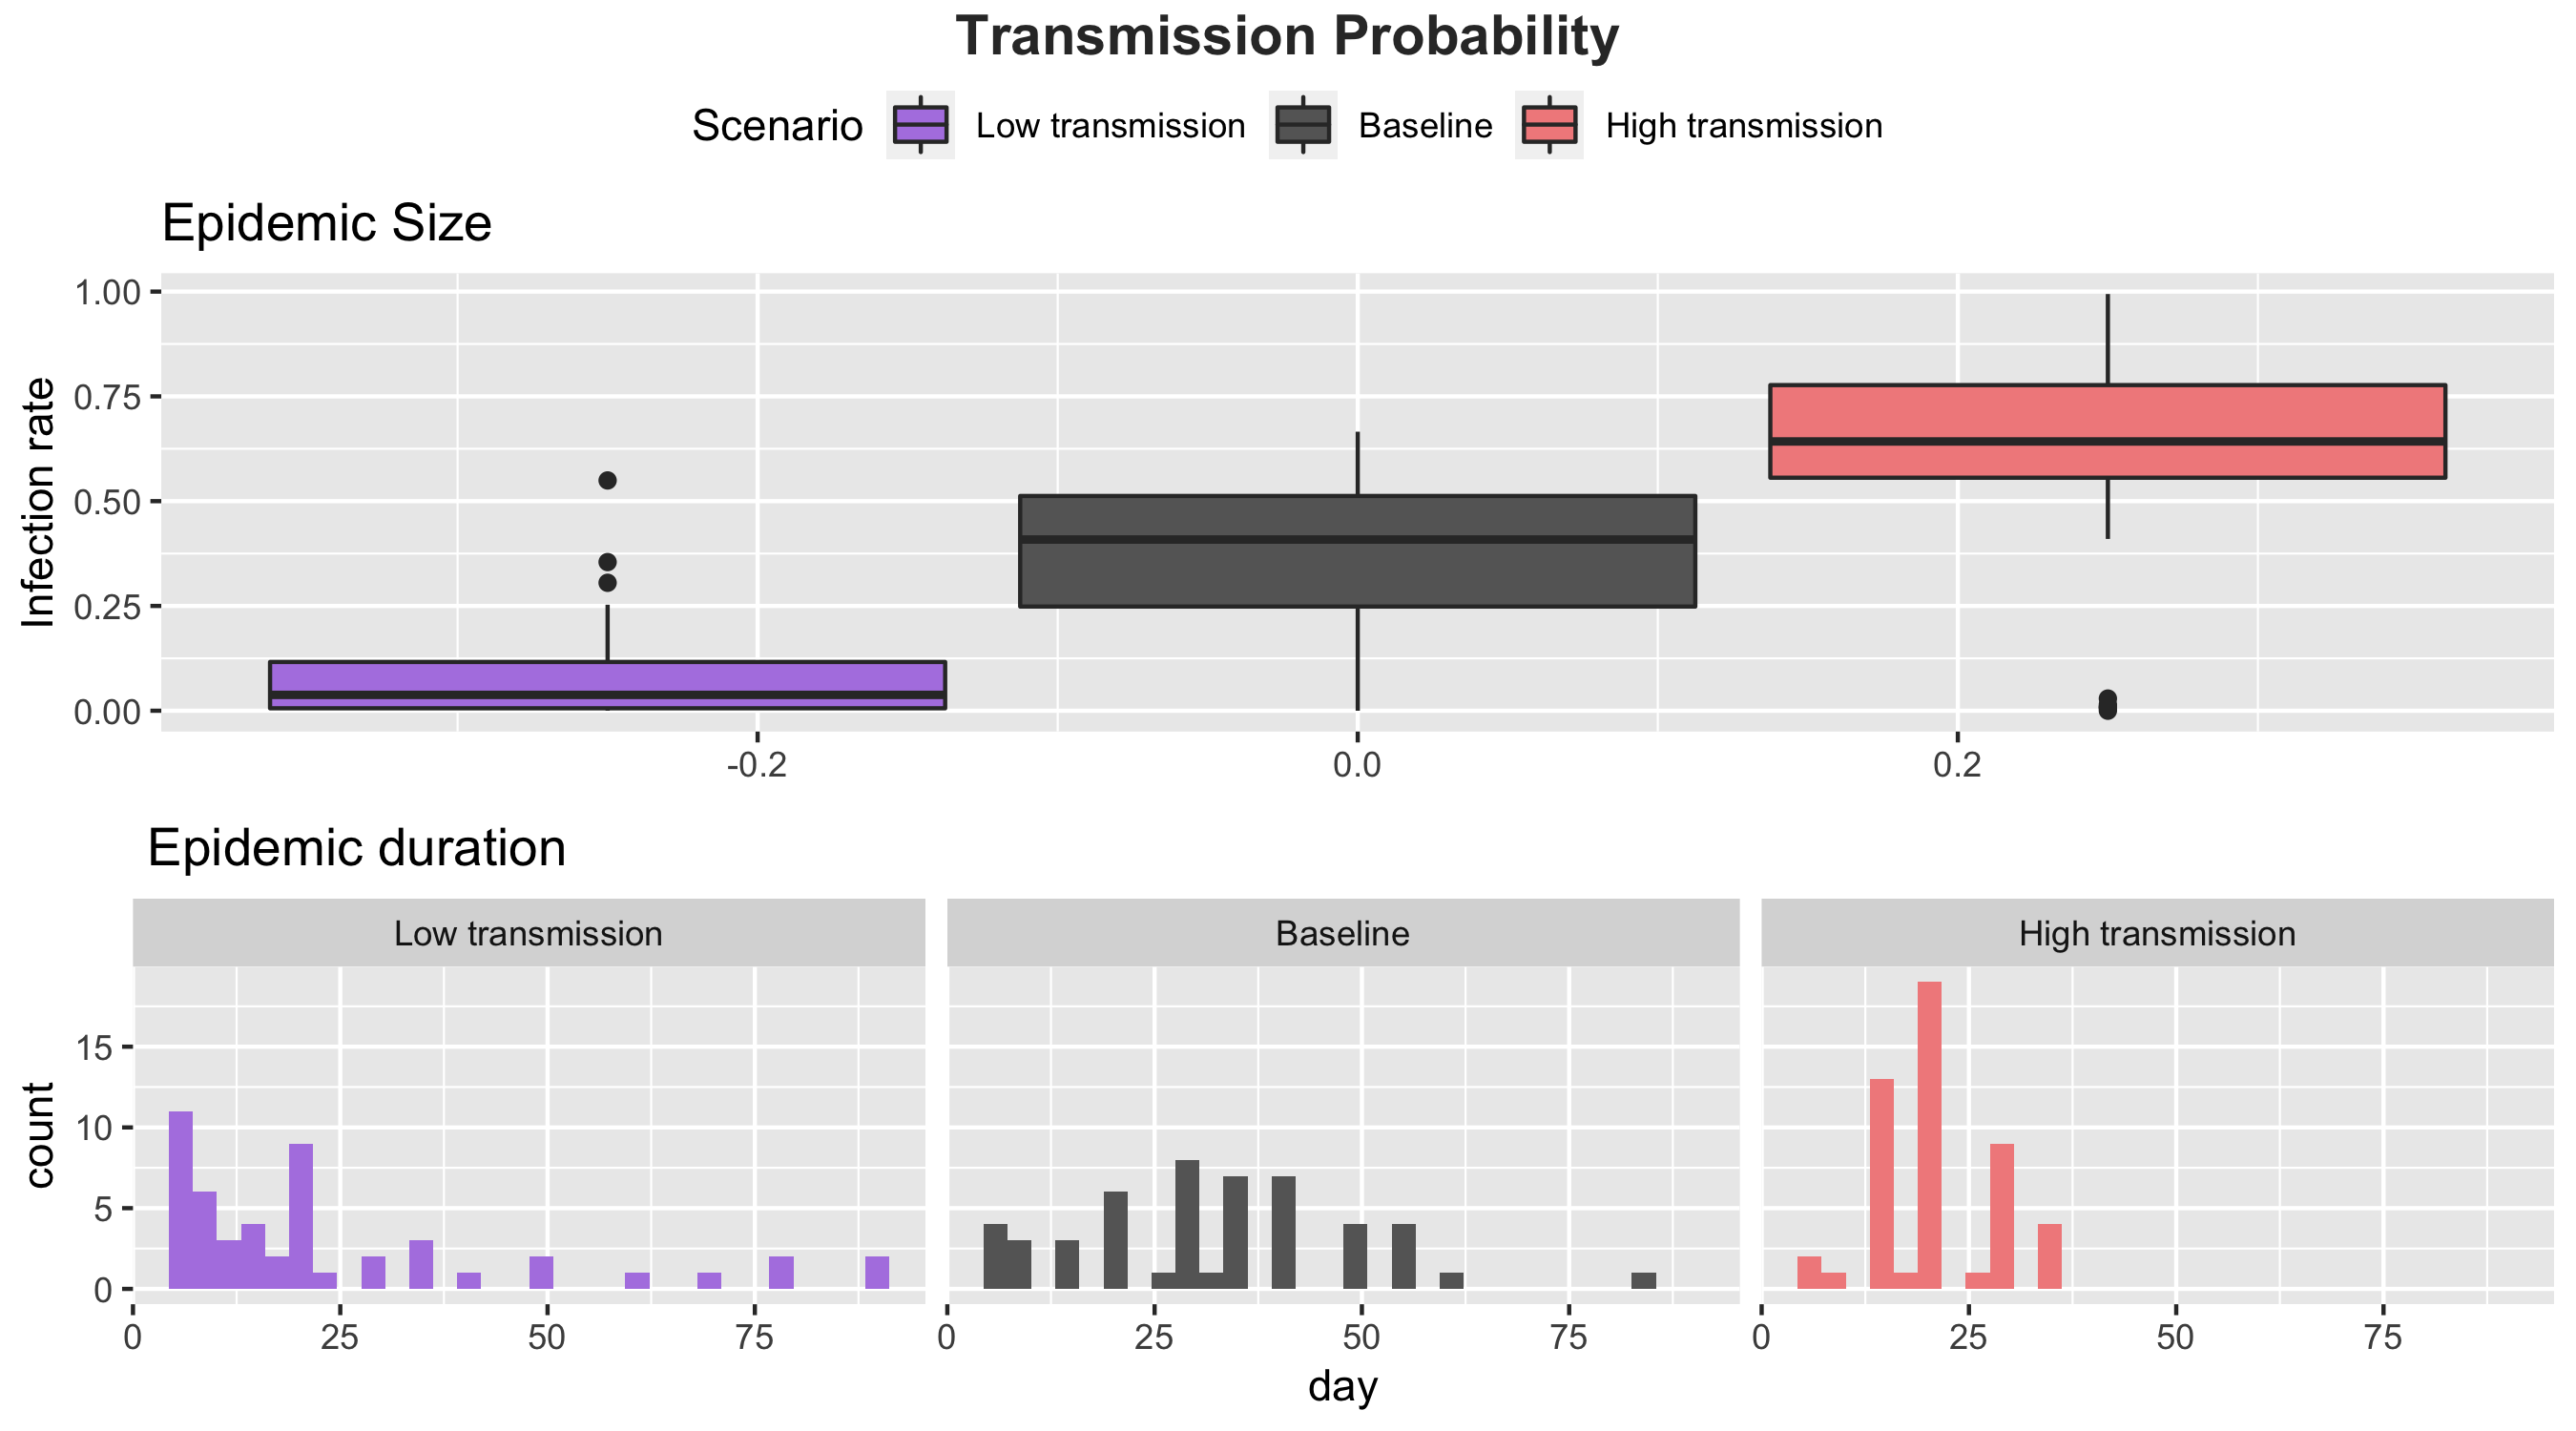
\includegraphics{Figures/SensitivityAnalysis/Transmission}\\
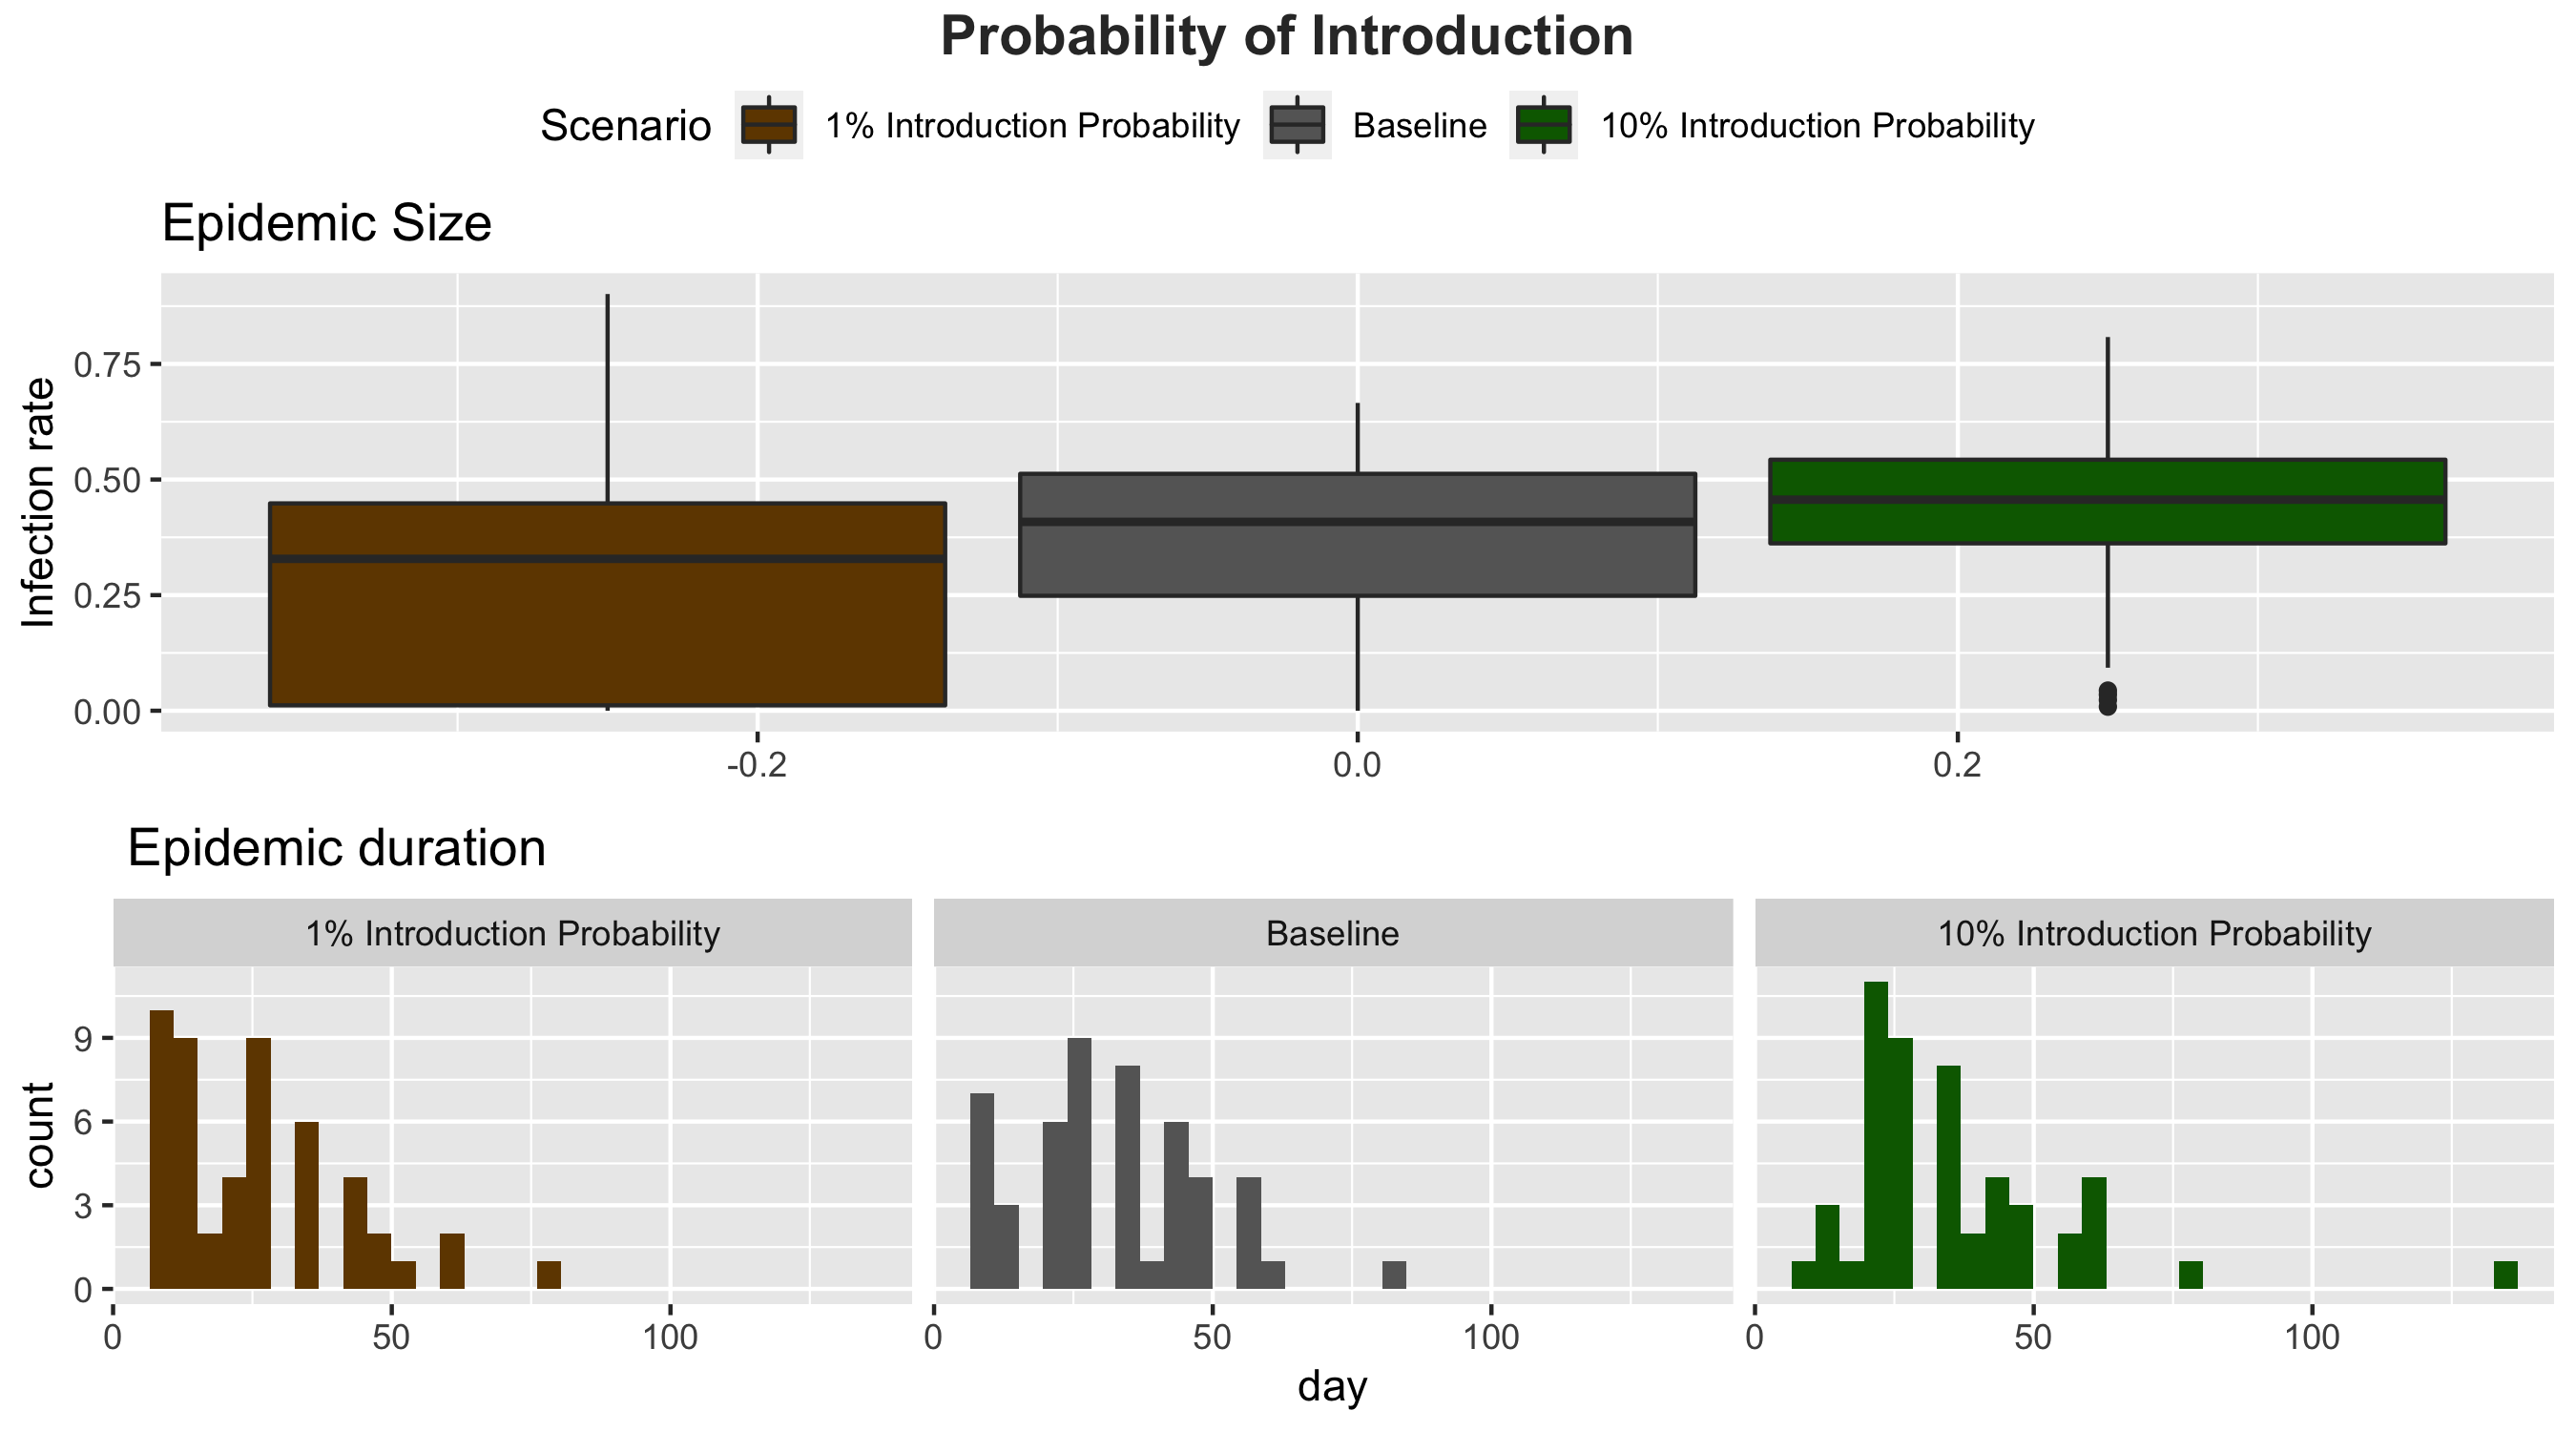
\includegraphics{Figures/SensitivityAnalysis/Introduction}\\
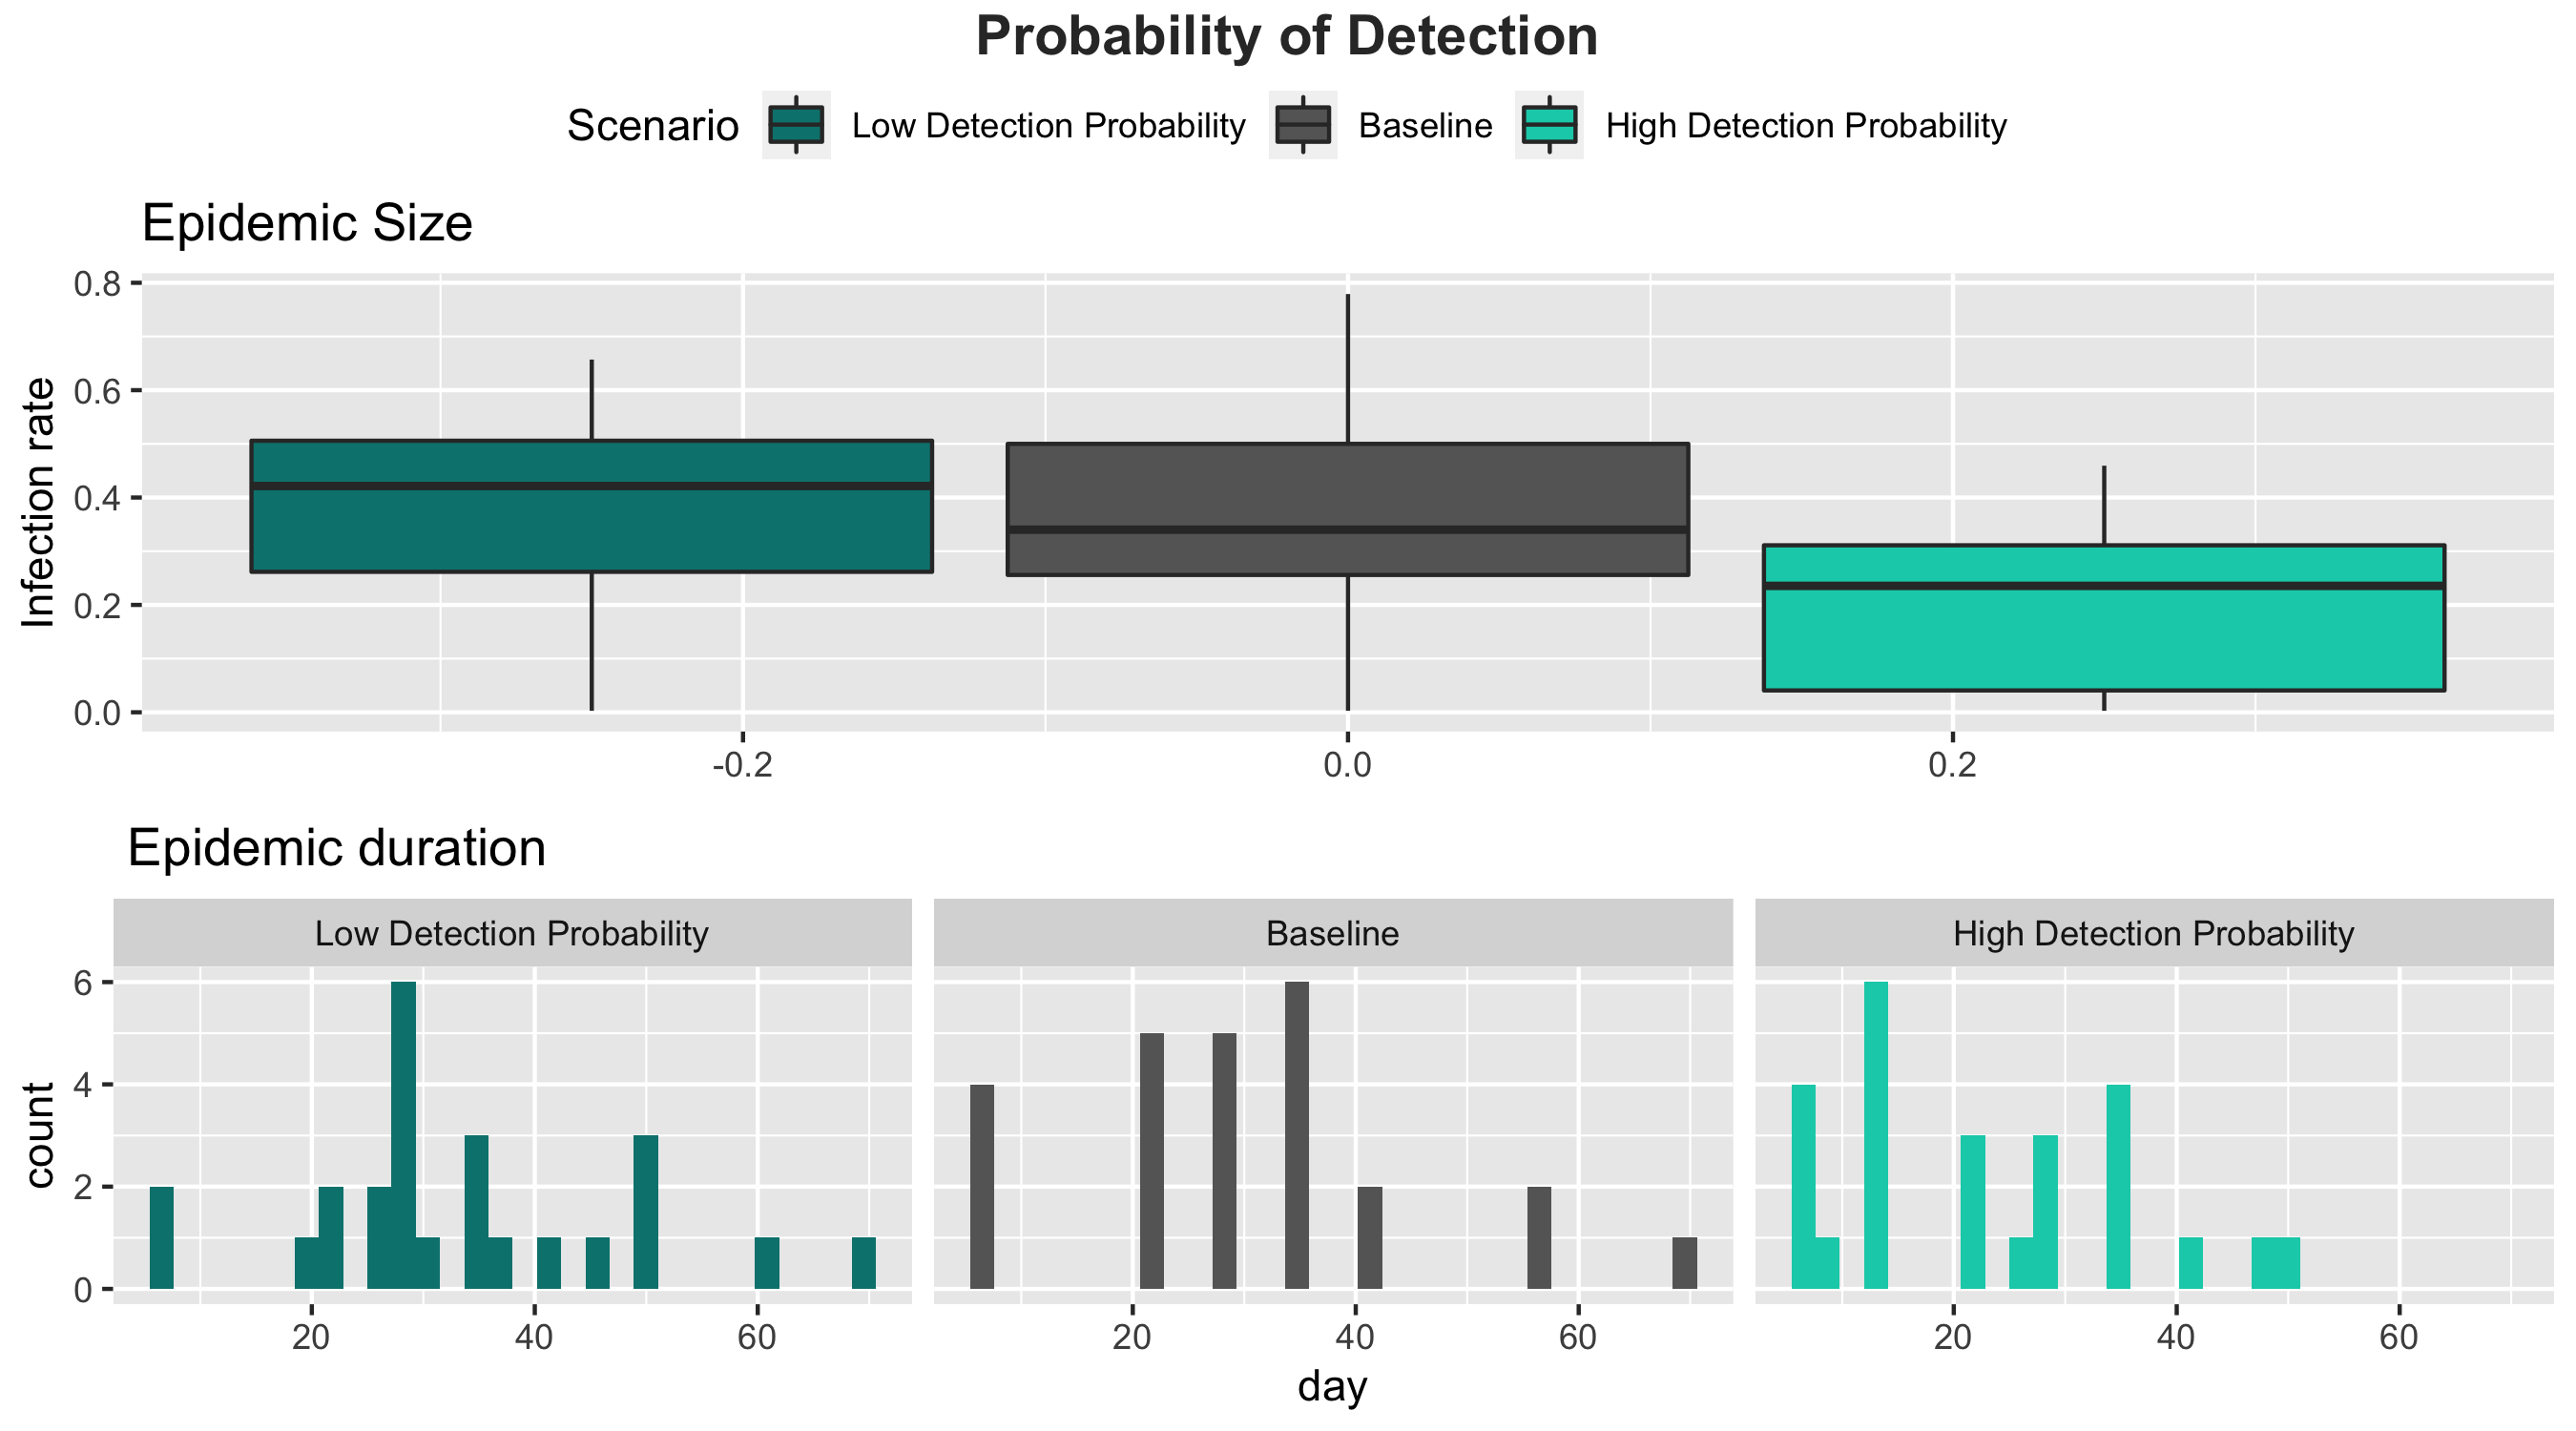
\includegraphics{Figures/SensitivityAnalysis/ProbDetection}\\
~\\
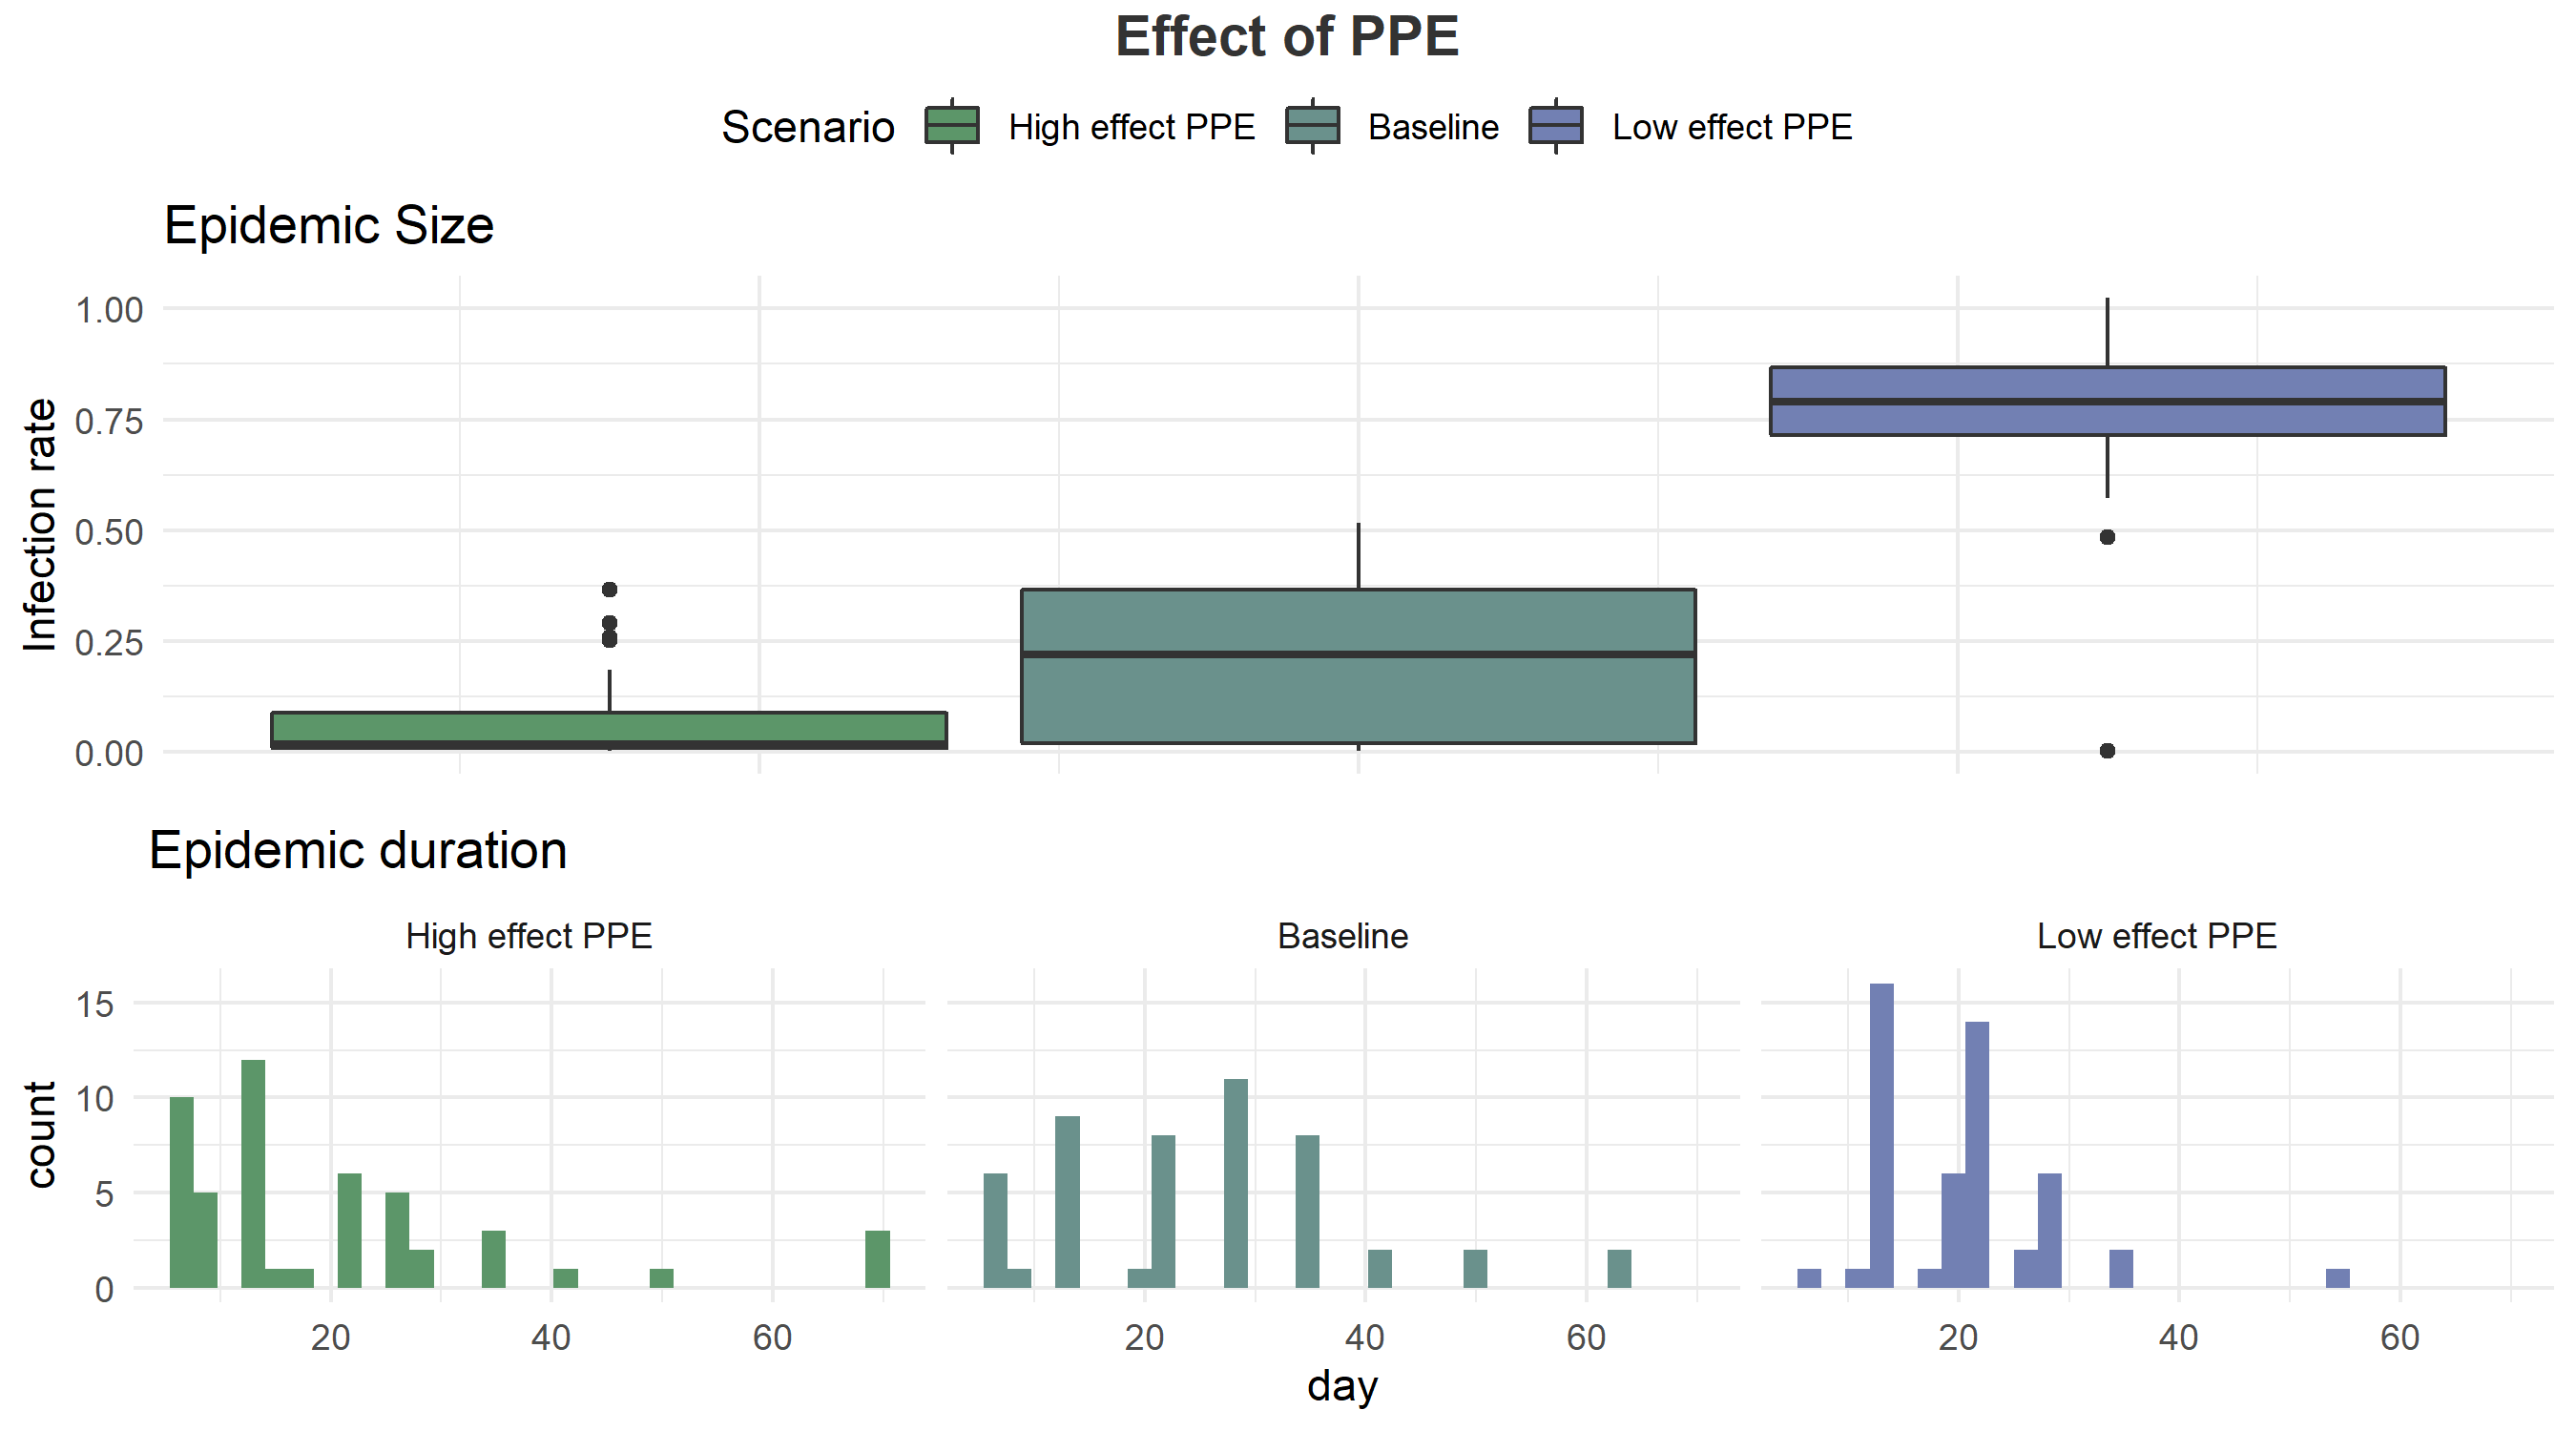
\includegraphics{Figures/SensitivityAnalysis/PPE}

\hypertarget{scenario-modeling-1}{%
\subsection{Scenario modeling}\label{scenario-modeling-1}}

\begin{itemize}
\tightlist
\item
  Strategic vaccination, focus on staff
\item
  Testing every 2 weeks
\item
  Testing every week
\item
  Is there a vaccination threshold
\end{itemize}

What happens if the vaccine is not as effective in older population? How
can we distribute the vaccine more effective? should we focus on staff?
When we focus on staff we block the staff resident transmission

balance between testing and vaccination. Who should get more tests?

\textbar Scenario\textbar{}

\hypertarget{references}{%
\section*{References}\label{references}}
\addcontentsline{toc}{section}{References}

\hypertarget{refs}{}
\begin{cslreferences}
\leavevmode\hypertarget{ref-Baden2020}{}%
Baden, Lindsey R., Hana M. El Sahly, Brandon Essink, Karen Kotloff,
Sharon Frey, Rick Novak, David Diemert, et al. 2020. ``Efficacy and
Safety of the mRNA-1273 SARS-CoV-2 Vaccine.'' \emph{New England Journal
of Medicine}, December, NEJMoa2035389.
\url{https://doi.org/10.1056/NEJMoa2035389}.

\leavevmode\hypertarget{ref-Chu2020}{}%
Chu, Derek K., Elie A. Akl, Stephanie Duda, Karla Solo, Sally Yaacoub,
Holger J. Schünemann, Amena El-harakeh, et al. 2020. ``Physical
distancing, face masks, and eye protection to prevent person-to-person
transmission of SARS-CoV-2 and COVID-19: a systematic review and
meta-analysis.'' \emph{The Lancet} 395 (10242): 1973--87.
\url{https://doi.org/10.1016/S0140-6736(20)31142-9}.

\leavevmode\hypertarget{ref-He2020}{}%
He, Xi, Eric H. Y. Lau, Peng Wu, Xilong Deng, Jian Wang, Xinxin Hao, Yiu
Chung Lau, et al. 2020. ``Temporal dynamics in viral shedding and
transmissibility of COVID-19.'' \emph{Nature Medicine} 26 (5): 672--75.
\url{https://doi.org/10.1038/s41591-020-0869-5}.

\leavevmode\hypertarget{ref-Pfizer2020}{}%
Pfizer-BioNTech. 2020. ``Vaccines and Related Biological Products
Advisory Committee Meeting December 10, 2020.'' Pfizer-BioNTech.

\leavevmode\hypertarget{ref-Polack2020}{}%
Polack, Fernando P, Stephen J Thomas, Nicholas Kitchin, Judith Absalon,
Alejandra Gurtman, Stephen Lockhart, John L Perez, et al. 2020. ``Safety
and Efficacy of the BNT162b2 mRNA Covid-19 Vaccine.'' \emph{The New
England Journal of Medicine}, 2603--15.
\url{https://doi.org/10.1056/NEJMoa2034577}.
\end{cslreferences}

\end{document}
